\documentclass[Rapport/Playerside/GameController/GameController.tex]{subfiles}
\label{sec:playerside_GameController_modultest}
\begin{document}
\subsubsection{Modultest}
I modultesten for GameController klassen blev klassen RPI\_IF brugt, da den allerede var færdig på det tidspunkt GameController klassen blev lavet. De eneste stubs, der skulle laves var til metoderne i CupLight\_IF og CupSensor\_IF. For at simulere en opdatering af kop status og hit status variablerne, blev de to metoder updateCupStatus og updateHitStatus kaldt via UART. Det vil sige at en UART komponent blev tilføjet projektet, som skulle tage et tastetryk fra tastaturet, hvorved en kombination af de funktioner ville blive kaldt sammen eller hver for sig med forskellige argumenter alt efter hvilken respons vi ønskede fra GameController klassen. For at simulerer CupLight\_IF's metoder blev funktionerne lavet med rigtige argumenter, men implementeringen består udelukkende af udskrivning til terminalen via UART. I funktionerne blev argumenter tilføjet, så man kan se, at de rigtige værdier ville blive kaldt, eller om funktionen overhovedet ville blive kaldt. Det første, der blev testet, var ændringen af states, hvorefter farvekoden for begge playersides blev testet(farvekoden blev også testet i RPI\_IF's modultest, men det blev bare gjort igen). Til sidst testes systemets respons state STARTING og PLAYING, når CupSensor\_IF ændrer kop status og hit status. I bilaget kan de forskellige kombinationer af tests ses, men nedenfor i figur \ref{fig:IDLE_STARTING} ses et eksempel, hvor setState bliver kaldt fra RPI\_IF klassen. Først med IDLE, hvor lysene slukkes(red, green og blue er 0) og herefter kaldes setState med STARTING, hvor controlling lights bliver kaldt. Heri bliver CupLight\_IF klassens metode controlLight kaldt 8 gange(blev ændret til 6 i færdige kode, da kun 6 kopper bliver brugt for hver playerside), som lyser rød hvilket er hvad missingColor variablen er i state STARTING, når Cupstatus er 0 på alle bits.
\begin{figure}
    \centering 
    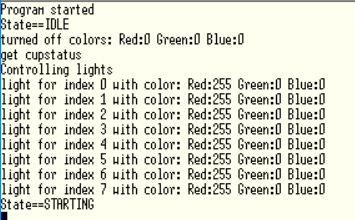
\includegraphics[width=0.5\linewidth]{Rapport/Playerside/graphics/GameController/IDLE_STARTING.PNG}
    \caption{Der skiftes her til state IDLE og herefter til state STARTING, man ser at lysene slukkes i IDLE, og i state STARTING og controllinglights bliver kaldt.}
    \label{fig:IDLE_STARTING}
\end{figure}
For at se flere kombinationer af tests med tastatur tryk i forskellige states henvises der til modultest for GameController klassen i afsnit \fullref{sec:GameController_modultest_bilag} i bilag.
\end{document}